% The left fixed point of a uniform MPS: l E = lambda l, where E is the
% transfer matrix -- A and its conjugate joined along the physical index.
%
% 07 draws this by hand, twice, to compare where the physical index leaves a
% triangle. This is the same equation on the grid, which takes it from the
% corner of the flat side: the triangle is set across in its slot so that its
% flat side is the site's line, and the site is one line from the ket to the
% bra, continuing that side.
%
% Two stacks and an equals sign, and the right-hand side is a stack with no
% sites: the environment alone, with its two indices ending where the first
% site's tensors would be. Those ends and the open indices of the left-hand
% side are at the same heights because both stacks have the same layers, not
% because anything was lined up.
\documentclass[border=4pt]{standalone}
\usepackage{amsmath,amssymb}
\usepackage{tikz-tensors}
\input{notation}
\begin{document}
\begin{tikzpicture}
  \tnstack[left=$l$]{X}{1}{ket, bra}
  \tnlayer{X}{ket}{canl/$A$}
  \tnlayer{X}{bra}{canl/$\bar A$}
  \tnconnect{X}
  \tnopen{right}{X-ket-1, X-bra-1}
  \tneq[$\lambda$]
  \tnstack[left=$l$]{Y}{0}{ket, bra}
  \tnconnect{Y}
\end{tikzpicture}
\end{document}
